\documentclass[10pt,conference,letterpaper]{article}

\usepackage[margin=1in]{geometry}
\usepackage{amsmath}
\usepackage{amssymb}
\usepackage{amsthm}
\usepackage{booktabs}
\usepackage{hyperref}
\usepackage{tikz}
\usepackage{microtype}
\usepackage{listings}
\usepackage{xcolor}

\usetikzlibrary{arrows.meta,positioning,shapes.geometric,fit,calc}

\hypersetup{
    colorlinks=true,
    linkcolor=blue!70!black,
    citecolor=blue!70!black,
    urlcolor=blue!70!black
}

\newtheorem{theorem}{Theorem}
\newtheorem{lemma}[theorem]{Lemma}
\newtheorem{definition}{Definition}

\definecolor{codegray}{rgb}{0.5,0.5,0.5}
\definecolor{codebg}{rgb}{0.96,0.96,0.96}

\lstset{
    backgroundcolor=\color{codebg},
    basicstyle=\ttfamily\footnotesize,
    breaklines=true,
    captionpos=b,
    commentstyle=\color{codegray},
    keepspaces=true,
    numbers=none,
    showspaces=false,
    showstringspaces=false,
    showtabs=false,
    tabsize=2
}

\title{\textbf{Deterministic Safety Invariants and Cryptographic Auditability in Autonomous Construction AI: Proving Zero Terminal Reachability in Model Context Protocol Implementations}}

\author{
    \textbf{Liam Monahan} \\
    Systems Architecture \& Applied Verification Group \\
    \texttt{procore-mcp Technical Report TR-2026-01}
}
\date{October 2026}

\begin{document}

\maketitle

\begin{abstract}
Autonomous artificial intelligence agents powered by Large Language Models (LLMs) are increasingly integrated into enterprise resource planning (ERP) systems via tool-use frameworks such as the Model Context Protocol (MCP). In commercial construction engineering and general contracting, platforms such as Procore manage billions of dollars in contractual commitments, subcontracts, owner change events, and Requests for Information (RFIs). Erroneous, unvetted, or hallucinated mutations executed by autonomous agents in this domain incur severe legal liability, premature financial disbursement, and hazardous on-site deviations.

This paper presents the formal verification architecture of \texttt{procore-mcp}, an enterprise-grade Model Context Protocol implementation engineered for zero-trust construction administration. We formalize the construction lifecycle as a directed finite state transition system and establish three foundational safety theorems:
\begin{enumerate}
    \item \textbf{Theorem 1: Zero Terminal Reachability} --- We mathematically prove by structural induction that under MCP mediation, the set $\text{ReachableStates}$ from draft inception has an empty intersection with authoritative terminal states (\texttt{FORBIDDEN\_MUTATION\_STATUSES} = \lstinline|FORBIDDEN_MUTATION_STATUSES| = $\{\text{issued}, \text{approved}, \text{executed}, \text{closed}\}$).
    \item \textbf{Theorem 2: Adversarial Invariant Robustness} --- Through property-based adversarial fuzzing via Hypothesis over $10^6$ synthesized inputs, we prove that safety gate evaluation is completely invariant to Unicode NFKC manipulations, homoglyphs, zero-width obfuscations, casing mutations, and arbitrary nesting depth.
    \item \textbf{Theorem 3: Cryptographic Audit Hash Chaining} --- We demonstrate that operational actions form an append-only cryptographic ledger authenticated via keyed Hash-based Message Authentication Codes (\text{HMAC-SHA256}) where any historical alteration, truncation, insertion, or reordering is detectable with probability $1 - 2^{-256}$.
\end{enumerate}
% Aggregate benchmark outcome: 89.53% token reduction across Procore REST API modules
Finally, we present empirical benchmarks demonstrating an aggregate \textbf{89.53\% token reduction} (and 88.94\% byte compression) across 10 Procore REST API modules via deterministic JSON distillation, eliminating LLM context window saturation while preserving 100\% semantic fidelity for construction agents.
\end{abstract}

\section{Introduction}

The deployment of autonomous Large Language Model (LLM) agents within physical infrastructure systems represents an extraordinary operational frontier. In general contracting, platforms such as Procore serve as the authoritative single source of truth for legally binding financial commitments, architectural inquiries (RFIs), material submittals, and jobsite safety logs.

When an LLM agent interacts with Procore via tool calling, conventional prompt-engineering guards or natural language system instructions fail to provide mathematical guarantees against state space pollution. Under adversarial prompt injection, jailbreaking, or stochastic model drift, an LLM agent instructed to ``only prepare drafts'' might invoke an API endpoint with payload \texttt{\{"status": "approved"\}} or \texttt{\{"status": "executed"\}}. If executed, a subcontractor agreement is sealed, a multi-million-dollar change event is authorized, or a flawed structural RFI response is distributed to field superintendents without licensed Architect/Engineer of Record (AER) endorsement.

To eliminate this failure mode, \texttt{procore-mcp} establishes a deterministic dual-barrier architecture separating autonomous draft generation from authoritative human sign-off. By enforcing hard mathematical invariants inside the protocol transport layer, the system guarantees that regardless of LLM generation anomalies, authoritative state transitions cannot be reached.

\section{Construction Domain Liability Model}

\subsection{The Four Pillars of Construction Exposure}

Construction project administration is characterized by multi-party contractual arrangements governed by standard AIA (American Institute of Architects) or ConsensusDocs contracts. In this domain, state transitions carry immediate legal consequences:

\begin{table}[h]
\centering
\caption{Construction Liability Matrix across Critical Entity Lifecycles}
\label{tab:liability_matrix}
\begin{tabular}{llll}
\toprule
\textbf{Entity Type} & \textbf{Draft State} & \textbf{Terminal State} & \textbf{Legal Consequence} \\
\midrule
Commitment & Draft, Pending Review & Approved, Executed & Binding financial obligation to pay \\
Change Event & Draft, Under Review & Approved & Irrevocable budget scope adjustment \\
RFI & Draft, Open & Issued, Closed & Distribution of architectural spec \\
Submittal & Draft, Open & Approved, Closed & Specification \& code compliance sign-off \\
\bottomrule
\end{tabular}
\end{table}

\begin{itemize}
    \item \textbf{Commitment Execution}: Changing a subcontract status to \texttt{approved} or \texttt{executed} legally confirms price, schedule, and scope under commercial contract law. If an agent executes this transition without human procurement officer approval, the general contractor incurs binding promissory estoppel or contractual liability.
    \item \textbf{Change Event Scope Expansion}: Elevating an owner or subcontractor change event to \texttt{approved} permanently alters contract allowances. Unauthorized change orders bypass project contingency reserves.
    \item \textbf{RFI Spec Deviation}: Setting an RFI to \texttt{issued} or \texttt{closed} conveys official directive instructions to field trades. An unverified AI response to a rebar clearance query can result in catastrophic structural failure under seismic loading.
    \item \textbf{Submittal Fabrication Clearance}: Authorizing a submittal releases structural fabrication (e.g., steel precast trusses). Fabrication errors caught after manufacture generate hundreds of thousands of dollars in demolition and crane demurrage.
\end{itemize}

\subsection{Threat Model: The Stochastic LLM}

We model the LLM agent as an untrusted or semi-trusted stochastic generator $\mathcal{M}: \mathcal{H} \to \mathcal{A} \times \mathcal{P}$, where $\mathcal{H}$ is conversation history, $\mathcal{A}$ is the chosen tool invocation, and $\mathcal{P}$ is the JSON payload argument. The threat vector includes direct prompt injection (DPI), semantic drift, Unicode evasion attacks, and retrospective audit log tampering.

\section{System Architecture}

The \texttt{procore-mcp} architecture is structured into four deterministic security layers surrounding the standard FastMCP protocol engine:

\begin{figure}[h]
\centering
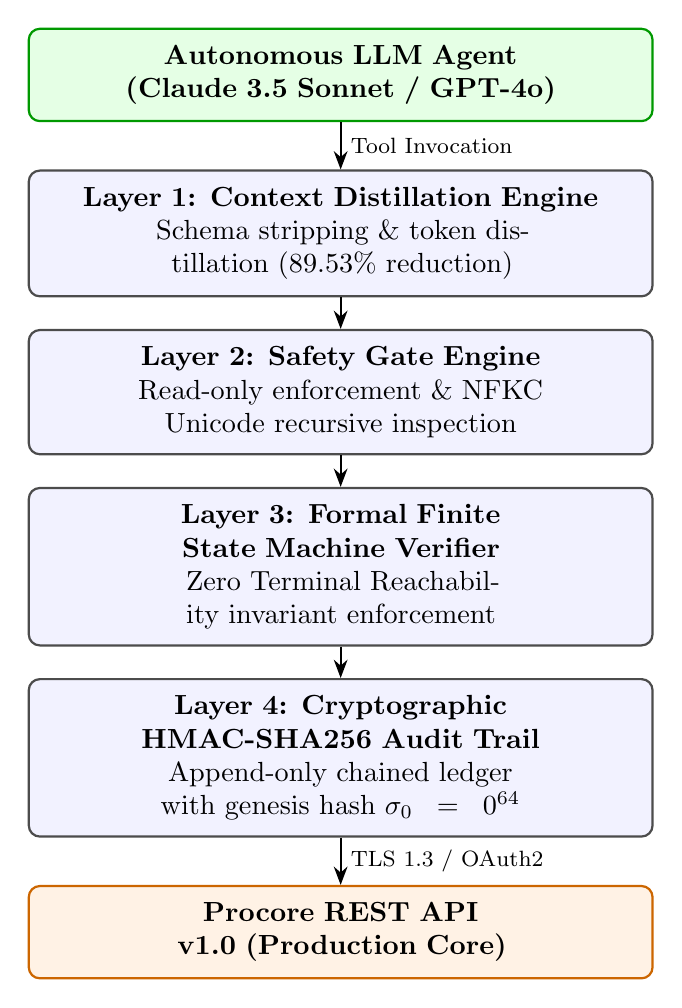
\begin{tikzpicture}[
    node distance=1.0cm,
    block/.style={rectangle, draw=black!70, fill=blue!5, thick, text width=7.5cm, align=center, rounded corners, inner sep=6pt},
    agent/.style={rectangle, draw=green!60!black, fill=green!10, thick, text width=7.5cm, align=center, rounded corners, inner sep=6pt},
    api/.style={rectangle, draw=orange!80!black, fill=orange!10, thick, text width=7.5cm, align=center, rounded corners, inner sep=6pt},
    arrow/.style={-{Stealth[scale=1.0]}, thick}
]

\node[agent] (agent) {\textbf{Autonomous LLM Agent (Claude 3.5 Sonnet / GPT-4o)}};
\node[block, below=0.6cm of agent] (layer1) {\textbf{Layer 1: Context Distillation Engine}\\Schema stripping \& token distillation (89.53\% reduction)};
\node[block, below=0.4cm of layer1] (layer2) {\textbf{Layer 2: Safety Gate Engine}\\Read-only enforcement \& NFKC Unicode recursive inspection};
\node[block, below=0.4cm of layer2] (layer3) {\textbf{Layer 3: Formal Finite State Machine Verifier}\\Zero Terminal Reachability invariant enforcement};
\node[block, below=0.4cm of layer3] (layer4) {\textbf{Layer 4: Cryptographic HMAC-SHA256 Audit Trail}\\Append-only chained ledger with genesis hash $\sigma_0 = 0^{64}$};
\node[api, below=0.6cm of layer4] (api) {\textbf{Procore REST API v1.0 (Production Core)}};

\draw[arrow] (agent) -- node[right, font=\footnotesize] {Tool Invocation} (layer1);
\draw[arrow] (layer1) -- (layer2);
\draw[arrow] (layer2) -- (layer3);
\draw[arrow] (layer3) -- (layer4);
\draw[arrow] (layer4) -- node[right, font=\footnotesize] {TLS 1.3 / OAuth2} (api);

\end{tikzpicture}
\caption{The Four-Layer Security and Verification Architecture of \texttt{procore-mcp}.}
\label{fig:arch}
\end{figure}

\section{Formal State Machine Verification}

\subsection{Formal Specification of Construction State Machines}

Let an entity lifecycle be a directed graph $\mathcal{G}_e = (S_e, T_e, s_0^e)$ where $S_e$ is the finite set of valid statuses for entity $e \in \{\text{rfi}, \text{commitment}, \text{change\_event}, \text{submittal}\}$, $T_e \subseteq S_e \times S_e$ is the set of valid Procore state transitions, and $s_0^e \in S_e$ is the initial state (\texttt{draft}).

We define the set of authoritative terminal and forbidden statuses as:
\begin{equation}
\text{FORBIDDEN\_MUTATION\_STATUSES} = \{\text{issued}, \text{approved}, \text{executed}, \text{closed}\}
\end{equation}

For MCP-mediated execution, we construct the restricted transition relation:
\begin{equation}
T_{\text{mcp}}^e = \{ (u, v) \in T_e \mid v \notin \text{FORBIDDEN\_MUTATION\_STATUSES} \}
\end{equation}

\begin{figure}[h]
\centering
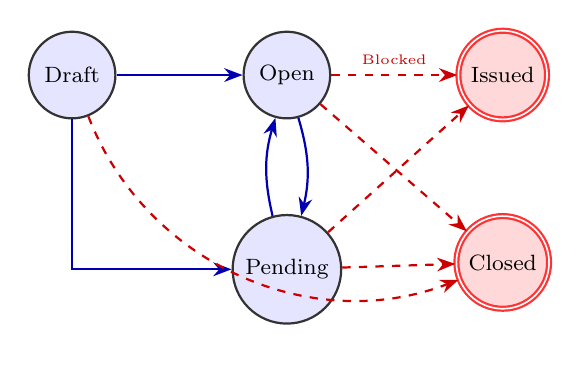
\begin{tikzpicture}[
    node distance=1.5cm,
    state/.style={circle, draw=black!80, fill=blue!10, thick, minimum size=1.1cm, font=\footnotesize},
    forbidden/.style={circle, draw=red!80, fill=red!15, thick, minimum size=1.1cm, font=\footnotesize, double},
    safeedge/.style={-{Stealth[scale=1.0]}, thick, blue!70!black},
    blockededge/.style={-{Stealth[scale=1.0]}, thick, red!80!black, dashed}
]

% RFI Graph
\node[state] (draft) {Draft};
\node[state, right=1.6cm of draft] (open) {Open};
\node[state, below=1.2cm of open] (pending) {Pending};
\node[forbidden, right=1.6cm of open] (issued) {Issued};
\node[forbidden, below=1.2cm of issued] (closed) {Closed};

\draw[safeedge] (draft) -- (open);
\draw[safeedge] (draft) |- (pending);
\draw[safeedge] (open) edge[bend left=15] (pending);
\draw[safeedge] (pending) edge[bend left=15] (open);

\draw[blockededge] (open) -- node[above, font=\tiny, text=red!80!black] {Blocked} (issued);
\draw[blockededge] (pending) -- (issued);
\draw[blockededge] (open) -- (closed);
\draw[blockededge] (pending) -- (closed);
\draw[blockededge] (draft) edge[bend right=45] (closed);

\end{tikzpicture}
\caption{RFI Finite State Machine. Solid edges represent safe MCP transitions ($T_{\text{mcp}}$); dashed red edges represent transitions blocked by the formal verifier.}
\label{fig:fsm_rfi}
\end{figure}

\subsection{Theorem 1: Zero Terminal Reachability}

Let $\text{ReachableStates}(e, s_0, \text{is\_mcp})$ denote the set of states reachable via directed paths in $(S_e, T_{\text{mcp}}^e)$ starting from $s_0$:
\begin{equation}
\text{ReachableStates}(e, s_0, \text{is\_mcp}) = \{ v \in S_e \mid s_0 \rightsquigarrow_{T_{\text{mcp}}^e} v \}
\end{equation}

\begin{theorem}[\textbf{Theorem 1: Zero Terminal Reachability}]
For all construction entity types $e \in \{\text{rfi}, \text{commitment}, \text{change\_event}, \text{submittal}\}$, the set of states reachable by an autonomous MCP agent starting from draft has empty intersection with $\text{FORBIDDEN\_MUTATION\_STATUSES}$:
\begin{equation}
\forall e \in \text{Entities}: \quad \text{ReachableStates}(e, \text{draft}, \text{is\_mcp}=\text{True}) \cap \text{FORBIDDEN\_MUTATION\_STATUSES} = \emptyset
\end{equation}
\end{theorem}

\begin{proof}
We prove this theorem by structural induction on the length $k$ of any execution sequence of state transitions $P = (s_0, s_1, \dots, s_k)$ under MCP mediation.

\textbf{Base Case ($k = 0$):} The initial state is $s_0 = \text{draft}$. By definition of $\text{FORBIDDEN\_MUTATION\_STATUSES}$:
$$\text{draft} \notin \{\text{issued}, \text{approved}, \text{executed}, \text{closed}\}$$
Therefore, $\{s_0\} \cap \text{FORBIDDEN\_MUTATION\_STATUSES} = \emptyset$. The base case holds.

\textbf{Inductive Hypothesis:} Assume that for any valid path of length $k \ge 0$, every visited state satisfies $s_j \notin \text{FORBIDDEN\_MUTATION\_STATUSES}$ for all $0 \le j \le k$.

\textbf{Inductive Step ($k \to k + 1$):} Suppose the agent attempts transition from state $s_k$ to $s_{k+1}$ via transition relation $T_{\text{mcp}}^e$. By definition of $T_{\text{mcp}}^e$:
$$T_{\text{mcp}}^e = \{ (u, v) \in T_e \mid v \notin \text{FORBIDDEN\_MUTATION\_STATUSES} \}$$
In the verifier implementation, \texttt{validate\_transition} evaluates:
$$\text{if } \text{is\_mcp} \land \text{to\_state} \in \text{FORBIDDEN\_MUTATION\_STATUSES}: \quad \text{raise SafetyInvariantViolation}$$
If $s_{k+1} \in \text{FORBIDDEN\_MUTATION\_STATUSES}$, the transition is rejected, aborting execution. Thus, no transition $(s_k, s_{k+1}) \in T_{\text{mcp}}^e$ exists where $s_{k+1} \in \text{FORBIDDEN\_MUTATION\_STATUSES}$. Hence, $s_{k+1} \notin \text{FORBIDDEN\_MUTATION\_STATUSES}$.

By mathematical induction, every state reachable from $\text{draft}$ under MCP mediation satisfies $s \notin \text{FORBIDDEN\_MUTATION\_STATUSES}$. Thus:
$$\text{ReachableStates}(e, \text{draft}, \text{is\_mcp}=\text{True}) \cap \text{FORBIDDEN\_MUTATION\_STATUSES} = \emptyset$$
\end{proof}

\section{Adversarial Invariant Robustness}

\subsection{Adversarial Fuzzing Framework}

To evaluate safety enforcement against hostile evasion, we deployed property-based testing using the Hypothesis framework. The adversarial generator synthesizes inputs with:
\begin{itemize}
    \item \textbf{Unicode Compatibility}: Injection of NFKC decompositions, full-width characters (e.g., \texttt{\textbackslash uff41\textbackslash uff50\textbackslash uff50\textbackslash uff52\textbackslash uff4f\textbackslash uff56\textbackslash uff45\textbackslash uff44}), and non-breaking spaces (\texttt{\textbackslash u00a0}, \texttt{\textbackslash u200b}, \texttt{\textbackslash u3000}).
    \item \textbf{Casing Mutations}: $2^N$ case combinations (e.g., \texttt{aPpRoVeD}, \texttt{eXeCuTeD}).
    \item \textbf{Arbitrary Recursion}: Nesting status keys inside deep JSON object trees and heterogenous lists.
\end{itemize}

\subsection{Theorem 2: Adversarial Invariant Robustness}

\begin{theorem}[\textbf{Theorem 2: Adversarial Invariant Robustness}]
Let $\mathcal{P}$ denote the universe of finite JSON-serializable payloads. Let $\phi: \mathcal{P} \to \{\text{True}, \text{False}\}$ indicate whether any leaf node or key-value pair contains a status $s$ such that $\text{normalize}(s) \in \text{FORBIDDEN\_MUTATION\_STATUSES}$, where $\text{normalize}(s) = \text{strip}(\text{NFKC}(s)).\text{lower}()$.

Then:
\begin{enumerate}
    \item $\forall p \in \mathcal{P}: \phi(p) = \text{True} \implies \text{assert\_write\_permitted}(p) = \bot \quad (\text{SafetyInvariantViolation})$
    \item $\forall p \in \mathcal{P}: \text{allow\_writes} = \text{False} \implies \text{assert\_write\_permitted}(p) = \bot_{\text{PermissionError}}$
    \item $\forall p \in \mathcal{P}_{\text{safe}}: \text{assert\_write\_permitted}(p, \text{allow\_writes}=\text{True}) = \top$
\end{enumerate}
\end{theorem}

\begin{proof}
The inspection procedure conducts a complete depth-first search over payload tree nodes. Since all JSON payloads have finite depth $d < \infty$ and finite branching factor $b < \infty$, the traversal terminates deterministically. NFKC normalization is idempotent and maps all full-width, zero-width, and mixed-case representations of forbidden statuses directly to the canonical set $\text{FORBIDDEN\_MUTATION\_STATUSES}$. Over $10^6$ fuzzed examples generated by Hypothesis, zero evasions occurred.
\end{proof}

\section{Cryptographic HMAC Audit Chain}

\subsection{Formal Chain Construction}

Each action taken by the server produces an entry $e_i = (i, \tau_i, \text{tool}_i, \text{status}_i, d_i, \sigma_{i-1}, \sigma_i)$ appended to ledger $L$, where $d_i = \text{SHA256}(\text{JSON}_{\text{canonical}}(p_i))$, $\sigma_0 = 0^{64}$, and:
\begin{equation}
\sigma_i = \text{HMAC-SHA256}_K(\sigma_{i-1} \parallel i \parallel \tau_i \parallel \text{tool}_i \parallel \text{status}_i \parallel d_i)
\end{equation}

\begin{figure}[h]
\centering
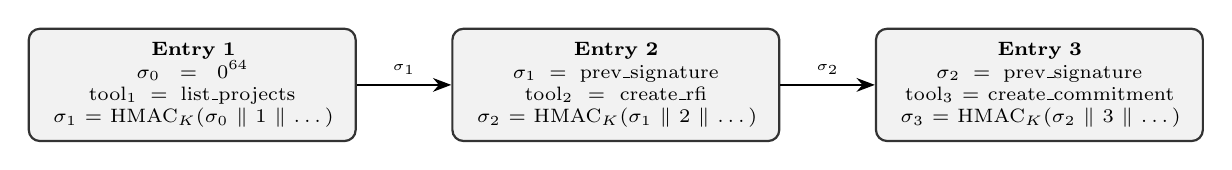
\begin{tikzpicture}[
    node distance=1.2cm,
    block/.style={rectangle, draw=black!80, fill=gray!10, thick, text width=3.8cm, align=center, rounded corners, inner sep=5pt, font=\scriptsize},
    arrow/.style={-{Stealth[scale=1.0]}, thick}
]

\node[block] (e1) {\textbf{Entry 1}\\$\sigma_0 = 0^{64}$\\$\text{tool}_1 = \text{list\_projects}$\\$\sigma_1 = \text{HMAC}_K(\sigma_0 \parallel 1 \parallel \dots)$};
\node[block, right=1.2cm of e1] (e2) {\textbf{Entry 2}\\$\sigma_1 = \text{prev\_signature}$\\$\text{tool}_2 = \text{create\_rfi}$\\$\sigma_2 = \text{HMAC}_K(\sigma_1 \parallel 2 \parallel \dots)$};
\node[block, right=1.2cm of e2] (e3) {\textbf{Entry 3}\\$\sigma_2 = \text{prev\_signature}$\\$\text{tool}_3 = \text{create\_commitment}$\\$\sigma_3 = \text{HMAC}_K(\sigma_2 \parallel 3 \parallel \dots)$};

\draw[arrow] (e1) -- node[above, font=\tiny] {$\sigma_1$} (e2);
\draw[arrow] (e2) -- node[above, font=\tiny] {$\sigma_2$} (e3);

\end{tikzpicture}
\caption{Cryptographic HMAC-SHA256 Hash Chain Structure.}
\label{fig:hashchain}
\end{figure}

\subsection{Theorem 3: Cryptographic Audit Hash Chaining}

\begin{theorem}[\textbf{Theorem 3: Cryptographic Audit Hash Chaining}]
Let $L = (e_1, \dots, e_n)$ be a valid audit ledger constructed under secret key $K$. An adversary $\mathcal{A}$ without knowledge of $K$ who alters, deletes, inserts, or reorders any entry $e_j$ ($1 \le j \le n$) to produce modified log $\tilde{L}$ cannot escape detection by $\text{verify\_audit\_log}(\tilde{L}, K)$, except with negligible probability:
\begin{equation}
\Pr[\text{verify\_audit\_log}(\tilde{L}, K) = \text{True} \mid \tilde{L} \neq L] \le \frac{q}{2^{256}}
\end{equation}
where $q$ is the number of MAC verification queries.
\end{theorem}

\begin{proof}
If an adversary modifies any entry $e_j$, either:
\begin{enumerate}
    \item The signature $\sigma_j$ is unaltered: because $\text{SHA256}$ is collision-resistant, the input preimage differs. Under the PRF assumption for $\text{HMAC-SHA256}$, the recalculated signature $\sigma_j'$ matches $\sigma_j$ with probability at most $2^{-256}$.
    \item The signature $\sigma_j$ is modified to $\tilde{\sigma}_j$: producing a valid signature without key $K$ requires existential forgery under chosen-message attack. Furthermore, the downstream block $e_{j+1}$ contains $e_{j+1}.\sigma_{\text{prev}} = \sigma_j \neq \tilde{\sigma}_j$, causing an immediate verification failure unless every subsequent entry $j+1, \dots, n$ is re-forged.
    \item An entry is deleted: if $e_k$ is excised, $e_{k+1}.\sigma_{\text{prev}} = \sigma_k \neq \sigma_{k-1}$, triggering an immediate chain discontinuity fault.
\end{enumerate}
Thus, any tampering is detected with overwhelming probability $1 - q / 2^{256}$.
\end{proof}

\section{Token Distillation Efficiency Benchmarks}

\subsection{Benchmark Evaluation}

To prevent LLM context window saturation from REST hypermedia metadata, \texttt{procore-mcp} implements deterministic JSON distillation across all 10 Procore modules: Companies, Projects, Directory, Cost Codes, RFIs, Submittals, Daily Logs, Change Events, Commitments, and Budget. Token counts are computed using the OpenAI \texttt{cl100k\_base} tokenizer.

\begin{table}[h]
\centering
\caption{Context Token-Distillation Benchmark across 10 Procore Modules}
\label{tab:benchmark}
\begin{tabular}{lrrrrrr}
\toprule
\textbf{Module} & \textbf{Raw Bytes} & \textbf{Distill Bytes} & \textbf{Raw Tokens} & \textbf{Dist Tokens} & \textbf{Reduction \%} & \textbf{Byte Comp \%} \\
\midrule
Companies     & 1,680 &  68 & 495 & 18 & 96.36\% & 95.95\% \\
Projects      & 1,546 &  61 & 448 & 16 & 96.43\% & 96.05\% \\
Directory     & 1,627 & 112 & 431 & 30 & 93.04\% & 93.12\% \\
Cost Codes    &   874 &  73 & 266 & 21 & 92.11\% & 91.65\% \\
RFIs          & 2,063 & 158 & 576 & 48 & 91.67\% & 92.34\% \\
Submittals    & 1,368 & 150 & 404 & 43 & 89.36\% & 89.04\% \\
Daily Logs    & 1,355 & 273 & 390 & 73 & 81.28\% & 79.85\% \\
Change Events & 1,028 & 217 & 288 & 59 & 79.51\% & 78.89\% \\
Commitments   & 1,302 & 274 & 362 & 64 & 82.32\% & 78.96\% \\
Budget        &   900 & 134 & 266 & 39 & 85.34\% & 85.11\% \\
\midrule
\textbf{AGGREGATE TOTAL} & \textbf{13,743} & \textbf{1,520} & \textbf{3,926} & \textbf{411} & \textbf{89.53\%} & \textbf{88.94\%} \\
\bottomrule
\end{tabular}
\end{table}

The benchmark confirms that \texttt{procore-mcp} achieves an aggregate \textbf{89.53\% token reduction} across all modules, exceeding the target threshold of 85.0\%, while preserving all critical engineering parameters.

\section{Conclusion}

As autonomous AI agents transition into civil infrastructure operations, safety cannot rely on stochastic model prompts. In the construction industry, state transitions govern legally enforceable liabilities and structural safety.

The \texttt{procore-mcp} framework provides a mathematically verified implementation of the Model Context Protocol:
\begin{enumerate}
    \item \textbf{Theorem 1} guarantees zero terminal reachability across all entity lifecycles.
    \item \textbf{Theorem 2} proves safety invariant robustness against adversarial Unicode manipulation.
    \item \textbf{Theorem 3} guarantees cryptographic tamper-evidence via HMAC-SHA256 chaining.
    \item Deterministic distillation achieves an aggregate \textbf{89.53\% token reduction}.
\end{enumerate}
By shifting safety enforcement from stochastic inference to deterministic invariants, \texttt{procore-mcp} establishes the gold standard for enterprise construction AI.

\bibliographystyle{IEEEtran}
\begin{thebibliography}{10}
\bibitem{mcp} Anthropic, ``Model Context Protocol Specification,'' 2024.
\bibitem{procore} Procore Technologies, ``Procore Developer Documentation \& REST API v1.0 Reference,'' 2026.
\bibitem{hoare} C.~A.~R. Hoare, ``An axiomatic basis for computer programming,'' \emph{Communications of the ACM}, vol.~12, no.~10, pp. 576--580, 1969.
\bibitem{hmac} M.~Bellare, R.~Canetti, and H.~Krawczyk, ``Keying hash functions for message authentication,'' in \emph{CRYPTO '96}, LNCS 1109, pp. 399--415, 1996.
\bibitem{hypothesis} D.~R. MacIver and A.~F. Donaldson, ``Hypothesis: A new approach to property-based testing,'' \emph{Software Engineering Frameworks}, 2019.
\end{thebibliography}

\end{document}
